\section{\bpfcontain{} Design and Implementation}
\label{sec:design}

Five specific goals informed the design of \bpfcontain{}'s policy language and
enforcement mechanism, enumerated below as Design Goals \ref{d:1} to \ref{d:5}.
%Note that there is a natural interplay between some of these design goals, while
%others are typically perceived as being in contention (specifically usability
%and security). In cases of conflict, it is essential to strike a careful balance
%between each property.

\begin{enumerate}[label=\bfseries D\arabic*., ref=D\arabic*, labelindent=1em]
  \item \label{d:1} \textsc{Usability.}
    \bpfcontain{}'s basic functionality should not impose unnecessary usability
    barriers on end-users.  Its policy language should be easy to understand and
    semantically meaningful to users without significant security knowledge. To
    accomplish this goal, \bpfcontain{} takes some inspiration from other high-level
    policy languages for containerized applications, such as those used in
    Snapcraft \cite{snap}.

  \item \label{d:2} \textsc{Configurability.}
    It should be easy for an end-user to reconfigure policy to match their
    specific use case, without worrying about the underlying details of the
    operating system or the policy enforcement mechanism. It should be possible
    to use \bpfcontain{} to restrict specific unwanted behaviour in a given
    application without needing to write a rigorous security policy from
    scratch.

  \item \label{d:3} \textsc{Transparency.}
    Containing an application using \bpfcontain{} should not require modifying the
    application's source code or running the application using a privileged SUID
    (Set User ID root) binary. \bpfcontain{} should be entirely agnostic to the rest
    of the system and should not interfere with its regular use.

  \item \label{d:4} \textsc{Adoptability.}
    \bpfcontain{} should be adoptable across a wide variety of system configurations
    and should not negatively impact the running system. It should be possible
    to deploy \bpfcontain{} in a production environment without impacting system
    stability and robustness or exposing the system to new security
    vulnerabilities. \bpfcontain{} relies on the underlying properties of its eBPF
    implementation to achieve its adoptability guarantees.

  \item \label{d:5} \textsc{Security.}
    \bpfcontain{} should be built from the ground up with security in mind. In
    particular, security should not be an opt-in feature and \bpfcontain{} should
    adhere to the principle of least privilege \cite{saltzer1975_protection} by
    default. It should be easy to tune a \bpfcontain{} policy to respond to new
    threats.
\end{enumerate}

\subsection{\bpfcontain{} Policy}
\label{sec:policy}

\bpfcontain{} policy consists of simple manifests written in YAML \cite{yaml},
a human-readable data serialization language based on key-value pairs.  Each
\bpfcontain{} container is associated with a manifest, which itself consists of
a few lines of metadata followed by a set of \textit{rights} and
\textit{restrictions}.  A \textit{right} specifies access that should be granted
to a container, while a \textit{restriction} is used revoke access. While rights
and restrictions may be combined at various levels of granularity, a restriction
\textit{always} overrides a right, without exception. In practice, this allows
the construction of nuanced policies that specify coarse-grained access with
finer-grained exceptions.  \Cref{tab:accesses} describes the various access
labels that can be used in \bpfcontain{} policy.

\begin{table}[htpb]
  \small
  \centering
  \caption{
    A list of resources which can be confined by \bpfcontain{} policy, along with their parameters and descriptions. Square brackets denote an optional parameter.
  }
  \label{tab:accesses}
  \begin{tabular}{llp{20em}}
  \toprule
  Resource              & Parameters          & Description \\
  \midrule
  \texttt{filesystem} & Mountpoint, [Access] &
    Grants or revokes access at the granularity of a filesystem mountpoint. Access defaults to \{read, write, append, chdir, setattr\}, unless otherwise specified. An optional \texttt{readonly} flag grants \{read, chdir\} access. \\
  \texttt{file}       & Pathname, Access  &
    Grants or revokes access at the granularity of individual files. Access must be specified. \\
  \midrule
  \texttt{capability} & Capability  &
    Grants or revokes access to the specified POSIX capability \todo{cite}. Note that this cannot be used to grant additional capabilities---it merely enforces on capabilities already granted to the process. \\
  \midrule
  \texttt{network}    & [Interface], [Access] &
    Grants or revokes access to network communications. A specific interface and access pattern may optionally be specified. \\
  \texttt{ipc}        & Container           &
    Grants or revokes access to communicate with processes in \textit{another} \bpfcontain{} container. This covers all supported System V IPC categories as well as signals. \\
  \midrule
  \texttt{tty}        & [Access]            &
    Grants or revokes access to \texttt{/dev/tty*} devices. \\
  \texttt{pts}        & [Access]            &
    Grants or revokes access to \texttt{/dev/pts/*} devices. \\
  \texttt{video}      & [Access]            &
    Grants or revokes access to \texttt{/dev/pts/video*} devices. \\
  \texttt{sound}      & [Access]            &
    Grants or revokes access to \texttt{/dev/pts/snd*} devices. \\
  \multicolumn{3}{c}{...} \\
  \bottomrule
  \end{tabular}
\end{table}

% TODO: Refer to this
\begin{table}[htpb]
  \small
  \centering
  \caption{
    Implicit policy in \bpfcontain{}, which is enforced regardless of a container's manifest. Implicit restrictions generally corresponds with resources which a well-behaved container should never need. Such accesses are generally recognized by the community as dangerous or enabling a container to escape confinement \todo{cite}. Implicit rights enable certain sane behaviours, such as interprocess communication between processes \textit{within} a container. These rights effectively constitute exceptions to ordinary enforcement. Note that implicit rights may still be overridden by an explicit restriction specified in the container's manifest.
  }
  \label{tab:implicit}
  \begin{tabular}{llp{25em}}
  \toprule
  Policy & Kind & Description \\
  \midrule
  BPF & Restriction &
    A container is disallowed from making \textit{any} \texttt{bpf(2)} system calls. This prevents it from loading, unloading, and accessing any eBPF programs and maps, including those which belong to \bpfcontain{} itself. \\
  Ptrace & Restriction &
    A container may not use \texttt{ptrace(2)} to trace or control processes. \\
  Lockdown & Restriction &
    A container is subject to fill lockdown \todo{cite} restrictions, disabling all operations that could be used for arbitrary code execution in the kernel. \\
  Kernel Modules & Restriction &
    A container may not load any modules into the kernel. \\
  Kexec & Restriction &
    A container may not use \texttt{kexec}-family system calls to load new kernels. \\
  Shutdown & Restriction &
    A container may not shut down or reboot the system. \\
  Key Management & Restriction &
    A container may not interface with the kernel's key management mechanisms. \\
  Quotactl & Restriction &
    A container cannot use the \texttt{quotactl(2)} system call to bypass restrictions on resource consumption. \\
  Rlimit & Restriction &
    A container cannot use the \texttt{getrlimit(2)}, \texttt{setrlimit(2)}, or \texttt{prlimit(2)} system calls to get or set resource limits. \\
  Scheduler & Restriction &
    A container cannot modify scheduling or I/O scheduling priority. \\
  Mount & Restriction &
    A container cannot mount, remount, unmount filesystems or move filesystem mounts. \\
  Pivot Root & Restriction &
    A container cannot pivot the root directory of a filesystem. \\
  Syslog & Restriction &
    A container cannot use the \texttt{syslog(2)} system call to access the kernel logs. \\
  Set Time & Restriction &
    A container cannot use the \texttt{settime(2)} system call to change the system time. \\
  \midrule
  IPC & Right &
    A process can always perform interprocess communication with another process within the same container. \\
  Procfs & Right &
    A process is granted full access to its own procfs entries, as well as those belonging to other processes within the same container. \\
  New Files & Right &
    A container is granted full access to any new files or directories that it creates. \\
  \bottomrule
  \end{tabular}
\end{table}

Following the principle of least privilege \cite{saltzer1975_protection},
\bpfcontain{} implements strict default-deny enforcement, only granting access
that the policy specifically declares under the container's set of rights. The
user may optionally change this behaviour and elect to enforce a default-allow
policy instead, by setting \lstinline[language=yaml]{default: allow} in the
manifest. A default-allow policy enables the easy restriction of specific
unwanted behaviour in a given program, without worrying about the details of
constructing a rigorous security policy.

\todo{Rework this, since the threat model section is now new} As a motivating example of \bpfcontain{} security policy, consider the Discord
client, discussed briefly in \Cref{subsection:threat_model}. Discord is a popular
cross-platform voice chat client designed for gamers and comes with an optional
feature, \enquote{Display Active Game}, which displays whatever game the user is
currently playing in their status message. To accomplish this, the Linux Discord
client periodically scans the \texttt{procfs} filesystem to obtain a list of all
running processes.  While this feature may seem innocuous at first glance, an
\texttt{strace} \cite{strace} of Discord reveals that it continually scans the
process tree even when the \enquote{Display Active Game} feature is
\textit{disabled}. This behaviour represents a gross violation of the user's
privacy expectations. To rectify this issue, a user might write a \bpfcontain{}
policy like the examples depicted in \Cref{lst:discord_a} and
\Cref{lst:discord_b}.

\begin{listing}[
  language=yaml,
  caption={
    A sample manifest for Discord \cite{discord} using \bpfcontain{}'s more
    restrictive default-deny confinement. All accesses which are not listed
    under the container's rights are implictly denied. The explicit restriction
    on access to \texttt{procfs} prevents Discord from scanning the process
    tree, regardless of its rights.
  },
  label={lst:discord_a},
  gobble=2]
  name: discord
  command: /bin/discord
  rights:
    - filesystem /
    - network
    - video
    - sound
  restrictions:
    - filesystem /proc
\end{listing}

\begin{listing}[
  language=yaml,
  caption={
    A sample manifest for Discord \cite{discord} using \bpfcontain{}'s optional
    default-allow confinement.  This permits a much simpler policy that directly
    targets Discord's \texttt{procfs} scanning behaviour.
  },
  label={lst:discord_b},
  gobble=2]
  name: discord
  command: /bin/discord
  default: allow
  restrictions:
    - filesystem /proc
\end{listing}

In the first example (\Cref{lst:discord_a}), the container grants access to the
root filesystem, networking capabilities, and video and sound devices. It
explicitly restricts access to the \texttt{procfs} filesystem, preventing
Discord from scanning the process tree. In the second example
(\Cref{lst:discord_b}), a more permissive policy is defined which serves
\textit{only} to restrict access to \texttt{procfs}. The choice of which
alternative to use is left entirely up to the user, and may depend on various
factors such as the existence of a pre-configured policy file, the desired use
case, and the user's level of comfort with \bpfcontain{}'s policy semantics.

To run a \bpfcontain{} container, the user invokes \texttt{bpfcontain run <name>} where
\texttt{name} is the unique container name declared in the manifest.  The
\texttt{bpfcontain run} command is a thin wrapper around that target application,
whose only purpose is to invoke a special library call,
\lstinline[language=c]|bpfcontain_confine|, that marks the process group for
confinement before executing the command(s) defined in the manifest.

An important feature of \bpfcontain{} is that the
\lstinline[language=c]|bpfcontain_confine| library call requires no additional
operating system privileges to start confinement.  This notion of unprivileged
confinement is a unique advantage over other container implementations in Linux.
Somewhat counter-intuitively, traditional container implementations often rely
on binaries with escalated privileges (e.g.~setuid root) to set up confinement.
Failure to correctly drop these elevated privileges may result in
\textit{escalation of privilege} in the host system, particularly if the
confined process manages to escape the container.  By obviating this need for
elevated privileges, \bpfcontain{} conforms with the principle of least
privilege and improves Linux containers' overall security.

As a side effect of \bpfcontain{}'s design, it is also possible for a generic
application to invoke the \lstinline[language=c]|bpfcontain_confine| library
call directly, eliminating the need to start the target application using the
\texttt{bpfcontain run} wrapper. This notion of self-confinement enables
application developers and package maintainers to ship \bpfcontain{} policy with
their software and enforce it transparently to the end-user. Since \bpfcontain{}
policy is designed to be readable and modifiable by end-users, a security policy
shipped with an application could optionally be tuned by the user according to
their specific needs.

%Besides the fact that it invokes a special library call, there is nothing
%special about the \texttt{bpfcontain run} wrapper---nothing is stopping a typical
%application from invoking \lstinline[language=c]|bpfcontain_confine()| directly, as
%it requires no special privileges. In this sense, one can also think of
%\bpfcontain{} as a mechanism for \textit{unprivileged self-confinement}.
%\Cref{sec:implementation} describes in detail the specifics of how \bpfcontain{}
%implements its confinement mechanism.

\subsection{Architecture}

\bpfcontain{} consists of both userspace and kernelspace components, which
interact co-operatively to implement the containerization and policy enforcement
mechanisms. Roughly, its architecture (depicted in \Cref{fig:architecture}) can
be broken down into the following four components:
\begin{enumerate}[label=\bfseries C\arabic*., ref=C\arabic*, labelindent=1em]

  \item \label{c:1}
  A privileged daemon, responsible for loading and managing the lifecycle of
  eBPF programs and maps, as well as logging security events to userspace.

  \item \label{c:2}
  A small shared library and unprivileged wrapper application used to initiate
  confinement.

  \item \label{c:3}
  A set of eBPF programs, running in kernelspace. These programs are attached to
  LSM hooks in the kernel as well as the shared library in \ref{c:2}.

  \item \label{c:4}
  A set of eBPF maps, special data structures which allow bidirectional
  communication between userspace and kernelspace. These maps are used to track
  the state of running containers and to store the active security policy for
  each container.
\end{enumerate}

\begin{figure}[htpb]
  \centering
  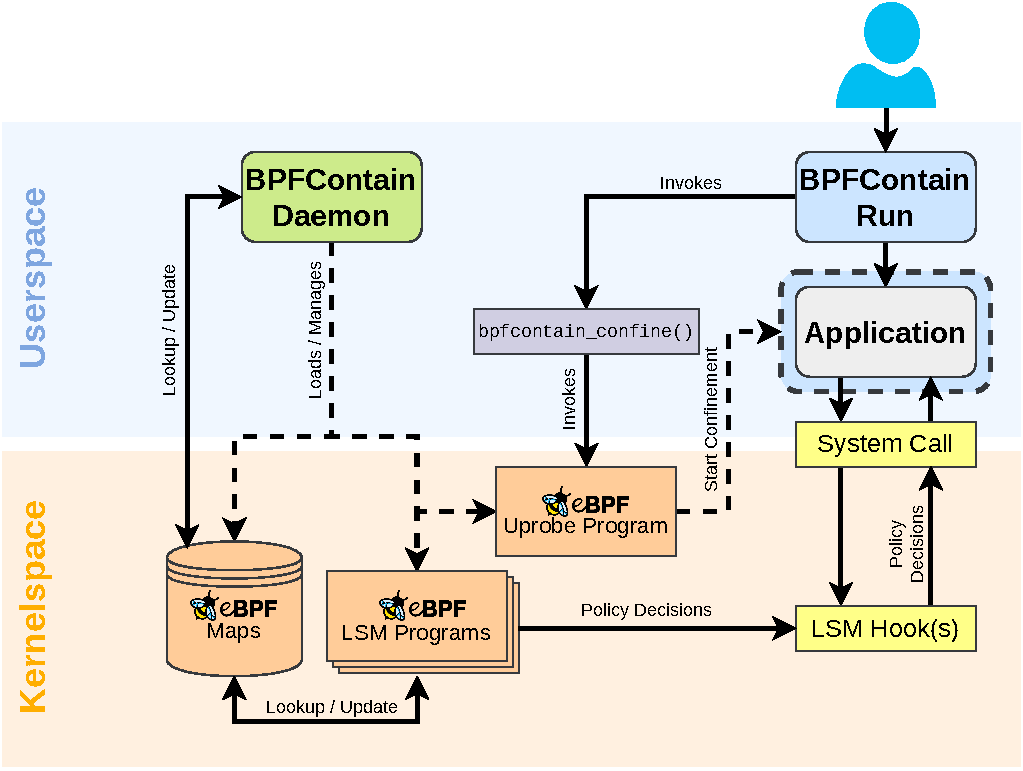
\includegraphics[width=1\linewidth]{figs/architecture.pdf}
  \caption{
    A diagram of \bpfcontain{}'s architecture. The privileged daemon (green) is
    responsible for loading the necessary eBPF maps and programs (orange) into
    the kernel and managing their lifecycle. The user starts a container by
    executing an unprivileged wrapper application (blue), which invokes the
    \texttt{bpfcontain\_confine} library call (purple), trapping to a special
    eBPF program that associates the process group with the correct policy.
    When the confined application (grey) makes a system call to request access
    to a sensitive resource, the kernel invokes one or more LSM hooks (yellow)
    which in turn trap to corresponding eBPF LSM programs that make the correct
    policy decision.
  }%
  \label{fig:architecture}
\end{figure}

%\bpfcontain{} consists of several userspace components written in the Python
%programming language and eBPF kernelspace components, written in a restricted
%subset of C.  In userspace, \bpfcontain{} runs a privileged daemon, \texttt{bpfcontain
%daemon}, which is responsible for loading eBPF programs into the kernel,
%creating and managing policy maps, and logging events to userspace. An
%unprivileged helper application, \texttt{bpfcontain run}, is used to run new
%containers.

In userspace, \bpfcontain{} runs in the background as a privileged daemon.  The
daemon is responsible for loading \bpfcontain{}'s eBPF programs and maps and
logging security events to userspace, such as policy violations.  When it first
starts, the daemon invokes a series of \texttt{bpf(2)} system calls to load its
eBPF programs and maps into the kernel. After loading all eBPF programs and
maps, the daemon then parses, translates, and loads each per-container policy
file into specialized policy maps.

To allow processes to request that they be placed into a container,
\bpfcontain{} attaches a specialized eBPF program type called a \texttt{uprobe}
(userspace probe) to a userspace library call, \texttt{bpfcontain\_confine}.
This function is a stub, whose only purpose is to trap to the uprobe---if this
function fails to trap the corresponding eBPF program (for example if
\bpfcontain{} has not yet loaded its eBPF programs into the kernel), this
function returns \texttt{-EAGAIN} to indicate that the caller should repeat the
request. Attaching a \texttt{uprobe} to a library call in this way is a common
eBPF design pattern, which effectively allows eBPF programs to make almost
arbitrary extensions to the kernel's API.

\subsection{Enforcing Policy}
\label{subsection:enforcing}

\bpfcontain{} enforces policy using eBPF programs attached to LSM hooks,
a feature introduced in Linux 5.7 by KP Singh's KRSI (Kernel Runtime Security
Instrumentation) patch \cite{singh2019_krsi,corbet2019_krsi}. KRSI enables the
attachment of multiple eBPF programs to a given LSM hook, which work
co-operatively with each other and other Linux security modules to come to
a policy decision, with any one denial resulting in a denial for the given
operation.

\bpfcontain{} only enforces security policy on processes which are currently
associated with a container. The list of processes associated with a container
is tracked using an eBPF map, which is updated whenever a process invokes the
\texttt{bpfcontain\_confine} library call (assuming it is not already in
a container), and whenever a process that is currently in a container forks
itself. Once a process has been associated with a container, it remains
associated with that container until it terminates.

Security policy in \bpfcontain{} falls into two categories: \textit{implicit}
and \textit{explicit}.  Implicit policy is the set of sensible defaults that are
defined to allow interaction \textit{within} a given container. For instance,
all processes in the same container may communicate with each other using
various interprocess communication mechanisms. Explicit policy, on the other
hand, refers to the rights and restrictions which have been explicitly defined
in a container's manifest. Unless a container has been marked as
\lstinline[language=yaml]|default: allow|, all access requests which are not
covered under the implicit or explicit policies for a container are denied by
default, and the access request is logged to userspace by the \bpfcontain{}
daemon.

\bpfcontain{} policy is stored in kernelspace using several eBPF maps, one for
each policy category. These maps are keyed using a composite key comprised of
a unique ID associated with each container combined with another unique
identifier for the given resource. For instance, filesystem policy is
keyed using the container's ID and the unique identifier associated with the
mounted device. Each key in a policy map is associated with a vector describing
the allowed access, depending on the granularity of the rule and its associated
parameters.

As instrumented LSM hooks are invoked, \bpfcontain{} queries the map of active
processes to determine which container the process is associated with, if any.
The corresponding policy map is then queried using the appropriate key, derived
from the container ID associated with the currently running process and the
unique identifiers corresponding to the requested resource. If no matching entry
is found, access is denied (assuming that the policy has not been marked default
allow).  Otherwise, the requested access is compared with the value found in the
map, and access is only granted if the values match.

